\documentclass[a4paper, 12pt]{article}

%%% Работа с русским языком
\usepackage{cmap}					% поиск в PDF
\usepackage{mathtext} 				% русские буквы в формулах
\usepackage[T2A]{fontenc}			% кодировка
\usepackage[utf8]{inputenc}			% кодировка исходного текста
\usepackage[russian]{babel}	% локализация и переносы

%%% Дополнительная работа с математикой
\usepackage{amsmath,amsfonts,amssymb,amsthm,mathtools} % AMS
\usepackage{icomma} % "Умная" запятая: $0,2$ --- число, $0, 2$ --- перечисление

%% Номера формул
%\mathtoolsset{showonlyrefs=true} % Показывать номера только у тех формул, на которые есть \eqref{} в тексте.

%% Шрифты
\usepackage{euscript}	 % Шрифт Евклид
\usepackage{mathrsfs} % Красивый матшрифт

%% Поля
\usepackage[left=2cm,right=2cm,top=2cm,bottom=2cm,bindingoffset=0cm]{geometry}

%% Русские списки
\usepackage{enumitem}
\makeatletter
\AddEnumerateCounter{\asbuk}{\russian@alph}{щ}
\makeatother

%%% Работа с картинками
\usepackage{graphicx}  % Для вставки рисунков
\graphicspath{{images/}{images2/}}  % папки с картинками
\setlength\fboxsep{3pt} % Отступ рамки \fbox{} от рисунка
\setlength\fboxrule{1pt} % Толщина линий рамки \fbox{}
\usepackage{wrapfig} % Обтекание рисунков и таблиц текстом

%%% Работа с таблицами
\usepackage{array,tabularx,tabulary,booktabs} % Дополнительная работа с таблицами
\usepackage{longtable}  % Длинные таблицы
\usepackage{multirow} % Слияние строк в таблице

%% Красная строка
\setlength{\parindent}{2em}

%% Интервалы
\linespread{1}
\usepackage{multirow}

%% TikZ
\usepackage{tikz}
\usetikzlibrary{graphs,graphs.standard}

%% Верхний колонтитул
\usepackage{fancyhdr}
\pagestyle{fancy}

%% Перенос знаков в формулах (по Львовскому)
\newcommand*{\hm}[1]{#1\nobreak\discretionary{}
	{\hbox{$\mathsurround=0pt #1$}}{}}

%% Мои дополнения
\usepackage{float} %Добавляет возможность работы с командой [H] которая улучшает расположение на странице
\usepackage{gensymb} %Красивые градусы
\usepackage{graphicx}               % Импорт изображений
\usepackage{caption} % Пакет для подписей к рисункам, в частности, для работы caption*
\usepackage{indentfirst}


\begin{document}

\newcommand{\HRule}{\rule{\linewidth}{0.7mm}} % Defines a new command for the horizontal lines, change thickness here
	
	\begin{center}
		\large\textbf{Московский Физико-Технический Институт}\\ % Name of your university/college
		\large\textbf{(государственный университет)}
	
		\vfill
		
		\Large Лабораторная работа по курсу общей физики № 4.5.3\\[0.5cm] % Preambule of your document title
		
		
		\HRule
		\\[0.4cm]
		{ \huge \bfseries Сканирующий интерферометр}% Title of your document
		\\[0.4cm] 
		\HRule
		\\[0.5cm]
		
		\ \\
	\textbf{\large Автор:} \\	
	\large Лепарский Роман Б01-003\\ % Your name and something more, your group num for example
		\vfill
		\hspace*{-0.8 cm}
\includegraphics[width=100 pt]{frkt_logo}\\ % logo of your  company/university/college
		\large Долгопрудный, 2022 % location and year
	\end{center}

\newpage
\setcounter{page}{2}
\fancyfoot[c]{\thepage}
\fancyhead[L] {Работа № 4.5.3} % some information in page header
\fancyhead[R]{}

\section{Аннотация}
\textbf{Цель работы}: исследовать явления дифракции Френеля и Фраунгофера на щели, изучить влияние дифракции на разрешающую способность оптических инструментов.


\textbf{В работе используются}: оптическая скамья, ртутная лампа, монохроматор, щели с регулируемой шириной, рамка с вертикальной нитью, двойная щель, микроскоп на поперечных салазках с микрометрическим винтом, зрительная труба.

\section{Теоретические сведения}
\subsection*{А. Дифракция Френеля}
\begin{figure}[H]
	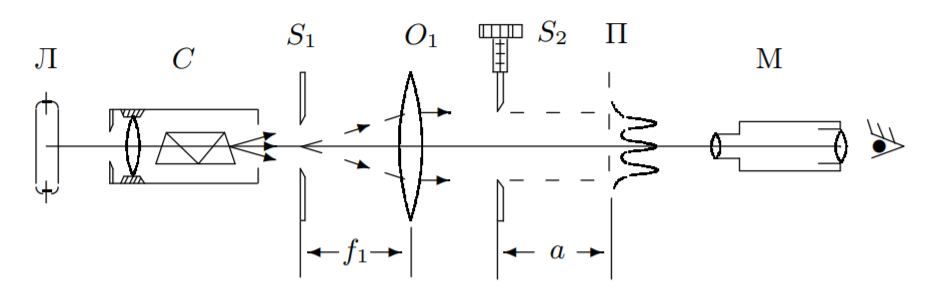
\includegraphics[scale=0.7]{0.png}
	\centering
	\caption{Схема установки 1.}
\end{figure}
При освещении $S_2$ параллельным пучком лучей (плоская зона) зоны Френеля представляют собой плоскости, параллельные краям щели. Результирующая амплитуда в точке наблюдения определеяется суперпозицией колебаний от тех зон Френеля, которые не перекрыты створками щели. Графическое определение результирующей амплитуды производится с помощью векторной диаграммы -- спирали Корню. Суммарная ширина $m$ зон Френеля $z_m$ определяется соотношение
\begin{equation}
z_m = \sqrt{am\lambda},
\end{equation}
где $a$ -- расстояние от щели до плоскости П. Вид наблюдаемой картины определяется количеством зон Френеля $\Phi$:
$$
\Phi^2 = \dfrac{D}{\sqrt{a\lambda}}
$$
Если их $m$, то будет набюдаться $m-1$ тёмная полоса.
\subsection*{Б. Дифракция Фраунгофера на щели}

Дифракцию Фраунгофера можно наблюдать на установке Рис. 1, но для удобства к подобной установке добавляется объектив $O_2$.

\begin{figure}[H]
	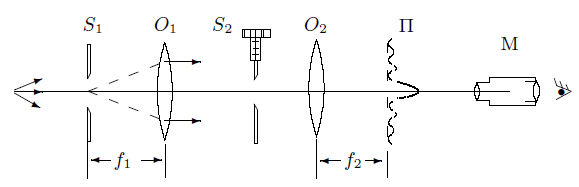
\includegraphics[width = 0.7\textwidth]{3.png}
	\centering
	\caption{Схема установки 2.}
\end{figure}
Дифракционная картина здесь наблюдается в фокальной плоскости объектива $O_2$. Каждому значению $\theta$ соответствует в этой плоскости точка, отстоящая от оптической оси на расстоянии 
\begin{equation}
X = f_2 \tan \theta \approx f_2 \theta.
\end{equation}
При $\theta = 0$ разность хода между лучами нулевая, поэтому в центре поля зрения дифракционный максимум. Первый минимум соответствует $\theta_1$ такому, что в точке наблюдения разность хода пробегаем все значения от 0 до $2\pi$. Аналогично рассуждая, для $m$-й полосы
\begin{equation}
\theta_m = \frac{m \lambda}{D}
\end{equation}
Расстояние $X_m$ тёмной полосы от оптической оси из (2) и (3)
\begin{equation}
X_m = f_2m\frac{\lambda}{D}
\end{equation}
\subsection*{В. Дифракция Фраунгофера для двух щелей}
Для наблюдения дифракции Фраунгофера на двух щелях $S_2$ заменим экраном Э с двумя щелями. При этом для оценки влияния ширины входной щели на чёткость вместо $S_1$ поставим щель с микрометрическим винтом.
\begin{figure}[H]
	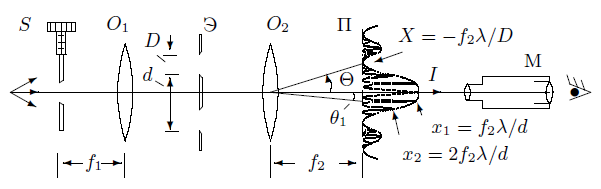
\includegraphics[width = 0.7\textwidth]{4.png}
	\centering
	\caption{Схема установки 3.}
\end{figure}
Два дифракционных изображения входной щели, одно из которых образовано лучами, прошедшими через левую, а другое -- через правую щели, накладываются друг на друга.
Светлая интерфереционная полоса наблюдается в случаях, когда разность хода равна целому числу длин волн. Таким образом, угловая координата максимума порядка $m$ равна
\begin{equation}
\theta_m = \dfrac{m \lambda}{d},
\end{equation}
где $d$ -- расстояние между щелями. Отсюда расстояние между соседними интерфереционными полосами в плоскости П равно
\begin{equation}
\delta x = f_2 \dfrac{\lambda}{d}
\end{equation}
Число интерференционных полос укладывающихся в области центрального максимума равна отношению ширины главного максимума $\frac{2\lambda f_2}{D}$ к расстоянию между соседними полосами:
\begin{equation}
n = \dfrac{2\lambda f_2}{D} \dfrac{1}{\delta f}= \dfrac{2d}{D}.
\end{equation}
При дифракции света на двух щелях чёткая система интерференционных полос наблюдается только при достаточно узкой ширине входной щели $S$. При увеличении ширины картинка пропадает и появляется вновь, но полосы при этом сильно размыты и видны плохо.
\subsection*{Г. Влияние дифракции на разрешающую способность оптического инструмента}
\begin{figure}[H]
	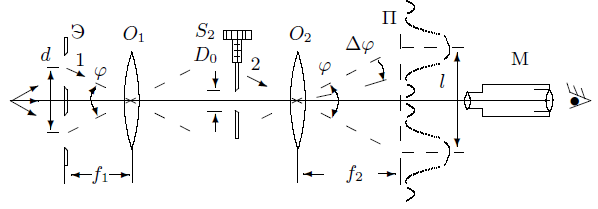
\includegraphics[width = 0.8\textwidth]{5.png}
	\centering
	\caption{Схема установки 4.}
\end{figure}
В отсутствие щели $S_2$ линзы $O_1$ и $O_2$ создают на плоскости П изоюражение щели $S_1$ и это изображение рассматриваются микроскопом М. Таким образом, установку можно рассматривать как оптический инструмент, предназначенные для получения изображения предмета. Если перед $O_2$ расположить $S_2$, то изображение объекта будет искажено из-за дифракции. Чем меньше ширина щели, тем сильнее искажение. Качественной характеристикой этого искажения может служить $\varphi_{min}$ --- минимальное угловое расстояние между объектами (источниками), которые всё ещё воспринимаются как раздельные. Поместим вместо $S_1$ экран Э с двумя щелями с расстоянием $d$. Тогда на $S_2$ будут падать два пучка света с углом
\begin{equation}
\varphi = \dfrac{d}{f_1}
\end{equation}
Из геометрии расстояние $l$ между изображениями щелей в плоскости П равно 
\begin{equation}
l = \varphi f_2 = d \dfrac{f_2}{f_1}.
\end{equation}
Ширина $\Delta \varphi$ определяется дифракцией на $S_2$. Условия, при которых изображения различимы разные для разных наблюдателей, поэтому используют \textit{критерий Рэлея} -- \textit{максимум одного дифракционного пятна должен совпадать с минимумом другого}. В наших условиях это значит, что угловая полуширина $\frac{\lambda}{D}$ равна угловому расстоянию $\frac{l}{f_2}$.
\section{Обработка результатов}
\subsection{Дифракция Френеля на щели}

	Длина волны для этой работы $\lambda = 578$ нм.

	Запишем ширину щели $S_2$, измеренную с помощью микрометрического винта и шкалы микроскопа.
	\[
		b_micro = 0,25\pm0,02 \text{ мм}
	\]
	\[
		b_scale = 0,26\pm0,01 \text{ мм}
	\]
	В первом случае погрешность обусловлена точному измерению положения открытия щели. Во втором случае взята половина ц.д.
	
	Запишем начальное положение микроскопа (дифракция не наблюдается)
	\[
		x_0 = 64,3\pm0,1 \text{ см}
	\]
	
	Запишем в таблицу координаты микроскопа в зависимости от количества темных полос, найдем для каждого случая величину $z_m$
	\begin{table}[H]
		\centering
		\begin{tabular}{|l|l|l|l|l|l|}
			\hline
			$m$        & 1    & 2    & 3    & 4    & 5    \\ \hline
			$x_m$, см  & 62,2 & 62,9 & 63,3 & 63,6 & 63,8 \\ \hline
			$a$, см    & 2,1  & 1,4  & 1    & 0,7  & 0,5  \\ \hline
			$z_m$, мкм & 110  & 120  & 130  & 120  & 120  \\ \hline
		\end{tabular}
	\end{table}
	Погрешность найдем по формуле
	\[
		\sigma_z = \frac{\sqrt{n\lambda}}{2\sqrt{a}}\cdot\sigma_a = 12\text{ мкм}
	\]
	
	Отложим эти значения на графике $z_m(m)$
	\begin{figure}[H]
		\centering
		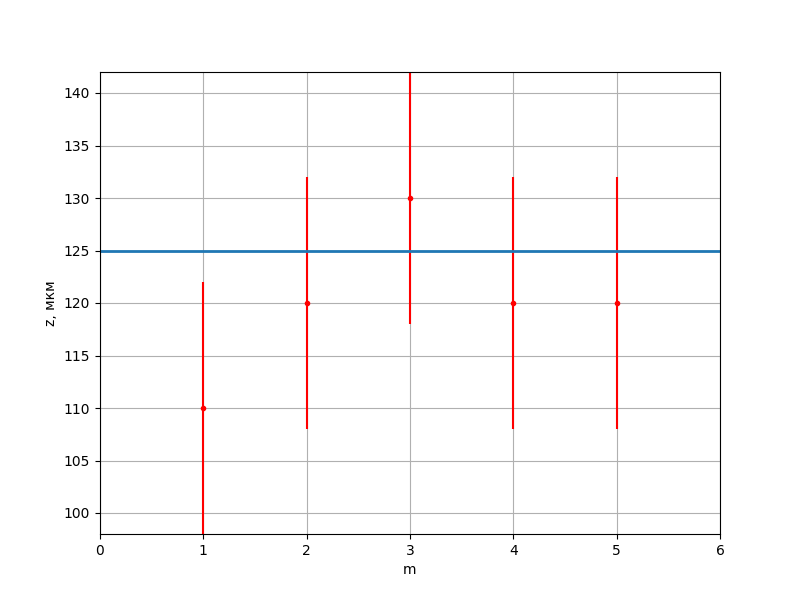
\includegraphics[scale = 0.7]{6}
	\end{figure}
	Линией на графике отмечена полуширина щели. Почти все значения лежат в пределах погрешности.
	
	\subsection{Дифракция Фраунгофера на щели}
	
	Ширина щели по показаниям микрометра: $b = 0,19\pm 0,01$ мм. Фокусное расстояние линзы $F_2 = 10,2 $ см. Запишем координаты минимумов дифракционной картины. Погрешность измерений $\sigma_X = 0,02$ мм обусловлена шириной темной полосы
	\begin{table}[H]
		\centering
		\begin{tabular}{|l|l|l|l|l|l|l|}
			\hline
			$m$       & -3   & -2   & -1   & 1    & 2    & 3    \\ \hline
			$X_m$, мм & 1,50 & 1,70 & 2,12 & 2,72 & 3,02 & 3,34 \\ \hline
		\end{tabular}
	\end{table}

	Построим график
	\begin{figure}[H]
		\centering
		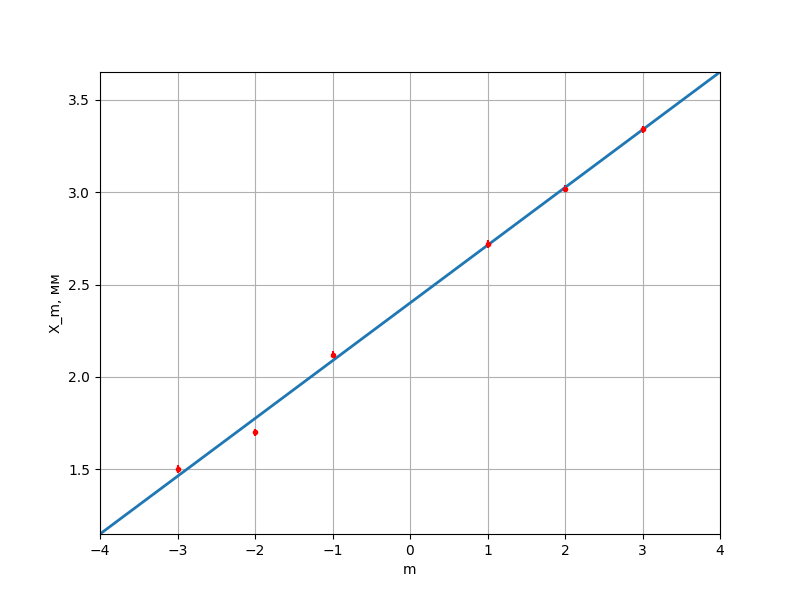
\includegraphics[scale = 0.7]{7}
	\end{figure}
	По МНК расстояние между минимумами $\Delta X = 0,312 \pm 0,007$ мм. Из формулы (4)
	\[
		b = \frac{\lambda}{\Delta X}F_2 = 0,188 \text{ мм}
	\]
	\[
		\sigma_b = \frac{\lambda}{\Delta X^2}F_2\cdot \sigma_{\Delta X} = 0,004 \text{ мм}
	\]
	Полученное значение совпадает с измеренным в пределах погрешности.

	\subsection{Дифракция Фраунгофера на двух щелях}
	
	Измерим координаты центрального максимума: $X_1 = 1,61\pm 0,01$ мм, $X_2 = 2,02\pm 0,01$ мм. Число светлых полос $n = 6\pm1$.
	\[
		\delta x = \frac{\Delta X}{n} = 0,07 \text{ мм}
	\]
	\[
		\sigma_{\delta x} = \sqrt{\left(\frac{1}{n}\sigma_{\Delta X}\right)^2+\left(\frac{\Delta X}{n^2}\sigma_n\right)^2} = 0,012\text{ мм}
	\]
	Рассчитаем величину $d$:
	\[
		d =\frac{\lambda}{\delta x}F_2 = 0,8 \text{ мм}
	\]
	\[
	\sigma_d = \frac{\lambda}{\delta x^2}F_2\cdot \sigma_{\delta x} = 0,14 \text{ мм}
	\]
	
	Дифракционная картина пропадает при раскрытии входной щели $b_0 = 0,071\pm0,03$ мм. Рассчитаем это значение по формуле:
	\[
		b_0 =\frac{\lambda}{d}F_2 = 0,07 \text{ мм}
	\]
	\[
	\sigma_{b_0} = \frac{\lambda}{d^2}F_2\cdot \sigma_{d} = 0,13 \text{ мм}
	\]
	Рассчитанное значение совпадает с экспериментальным в пределах погрешности.
	
	Из следующего пункта ширина щели $D = 0,2 \pm 0,11$ мм
	Соответственно количество полос
	\[
		n = \frac{2d}{D} = 8\pm4
	\]
	
	\subsection{Влияние дифракции на разрешающую способность}
	
	Запишем минимальную ширину щели $b_0 = 0,092\pm 0,003$ мм, при которой еще различимо изображение щели.
	
	Для проверки справедливости критерия Релея рассчитаем эту величину по формуле
	\[
		b_0 = \frac{\lambda}{d}F_1 = 0,08 \text{мм}
	\]
	\[
	\sigma_{b_0} = \frac{\lambda}{d^2}F_1\cdot \sigma_{d} = 0,03 \text{ мм}
	\]
	Полученное значение совпадает в пределах погрешности.
	
	Координаты краев двух щелей:
	\begin{table}[H]
		\centering
		\begin{tabular}{|l|l|l|l|l|}
			\hline
			$X$, мм & 0 & 0,12 & 0,84 & 1,18 \\ \hline
		\end{tabular}
	\end{table}

	\section{Вывод}
	В данной работе мы исследовали явление дифракции Френеля и Фраунгофера на щели и изучили влияние дифракции на разрешающую способность оптических приборов. 















 





	

\end{document}